\chapter{Desarrollo de la aplicación}

\epigraph{\textit{''Los programas deben ser escritos para que los lean las personas, y sólo incidentalmente, para que lo ejecuten las máquinas''}}{--- Abelson and Sussman}

Tras haber explicado en el capítulo anterior las diversas herramientas a usar para el desarrollo de la aplicación, en este capítulo se explicaran aspectos sobre el diseño de la aplicación y las diferentes decisiones tomadas a la hora de realizar dicho diseño.

El diseño de la aplicación es simple y minimista. El objetivo del proyecto consiste en hacer una aplicación lo más fácil de usar y con la mayor claridad posible de cara al usuario. Por ello, se ha optado por un enfoque que reduzca el numero de elementos al mínimo, además de que se adapta perfectamente a los estándares de diseño de Material Design\footnote{\url{https://material.io/design/}}, que son los recomendados a la hora de diseñar aplicaciones para Android.

\section{Interfaz gráfica}

Para la interfaz gráfica se ha optado por hacer un diseño primero en papel para después, en base a ese diseño y esa distribución de ventanas, elaborar en Android Studio toda la interfaz gráfica. Se puede observar un diseño primitivo en la siguiente imagen.

\begin{figure}[ht]
	\centering
	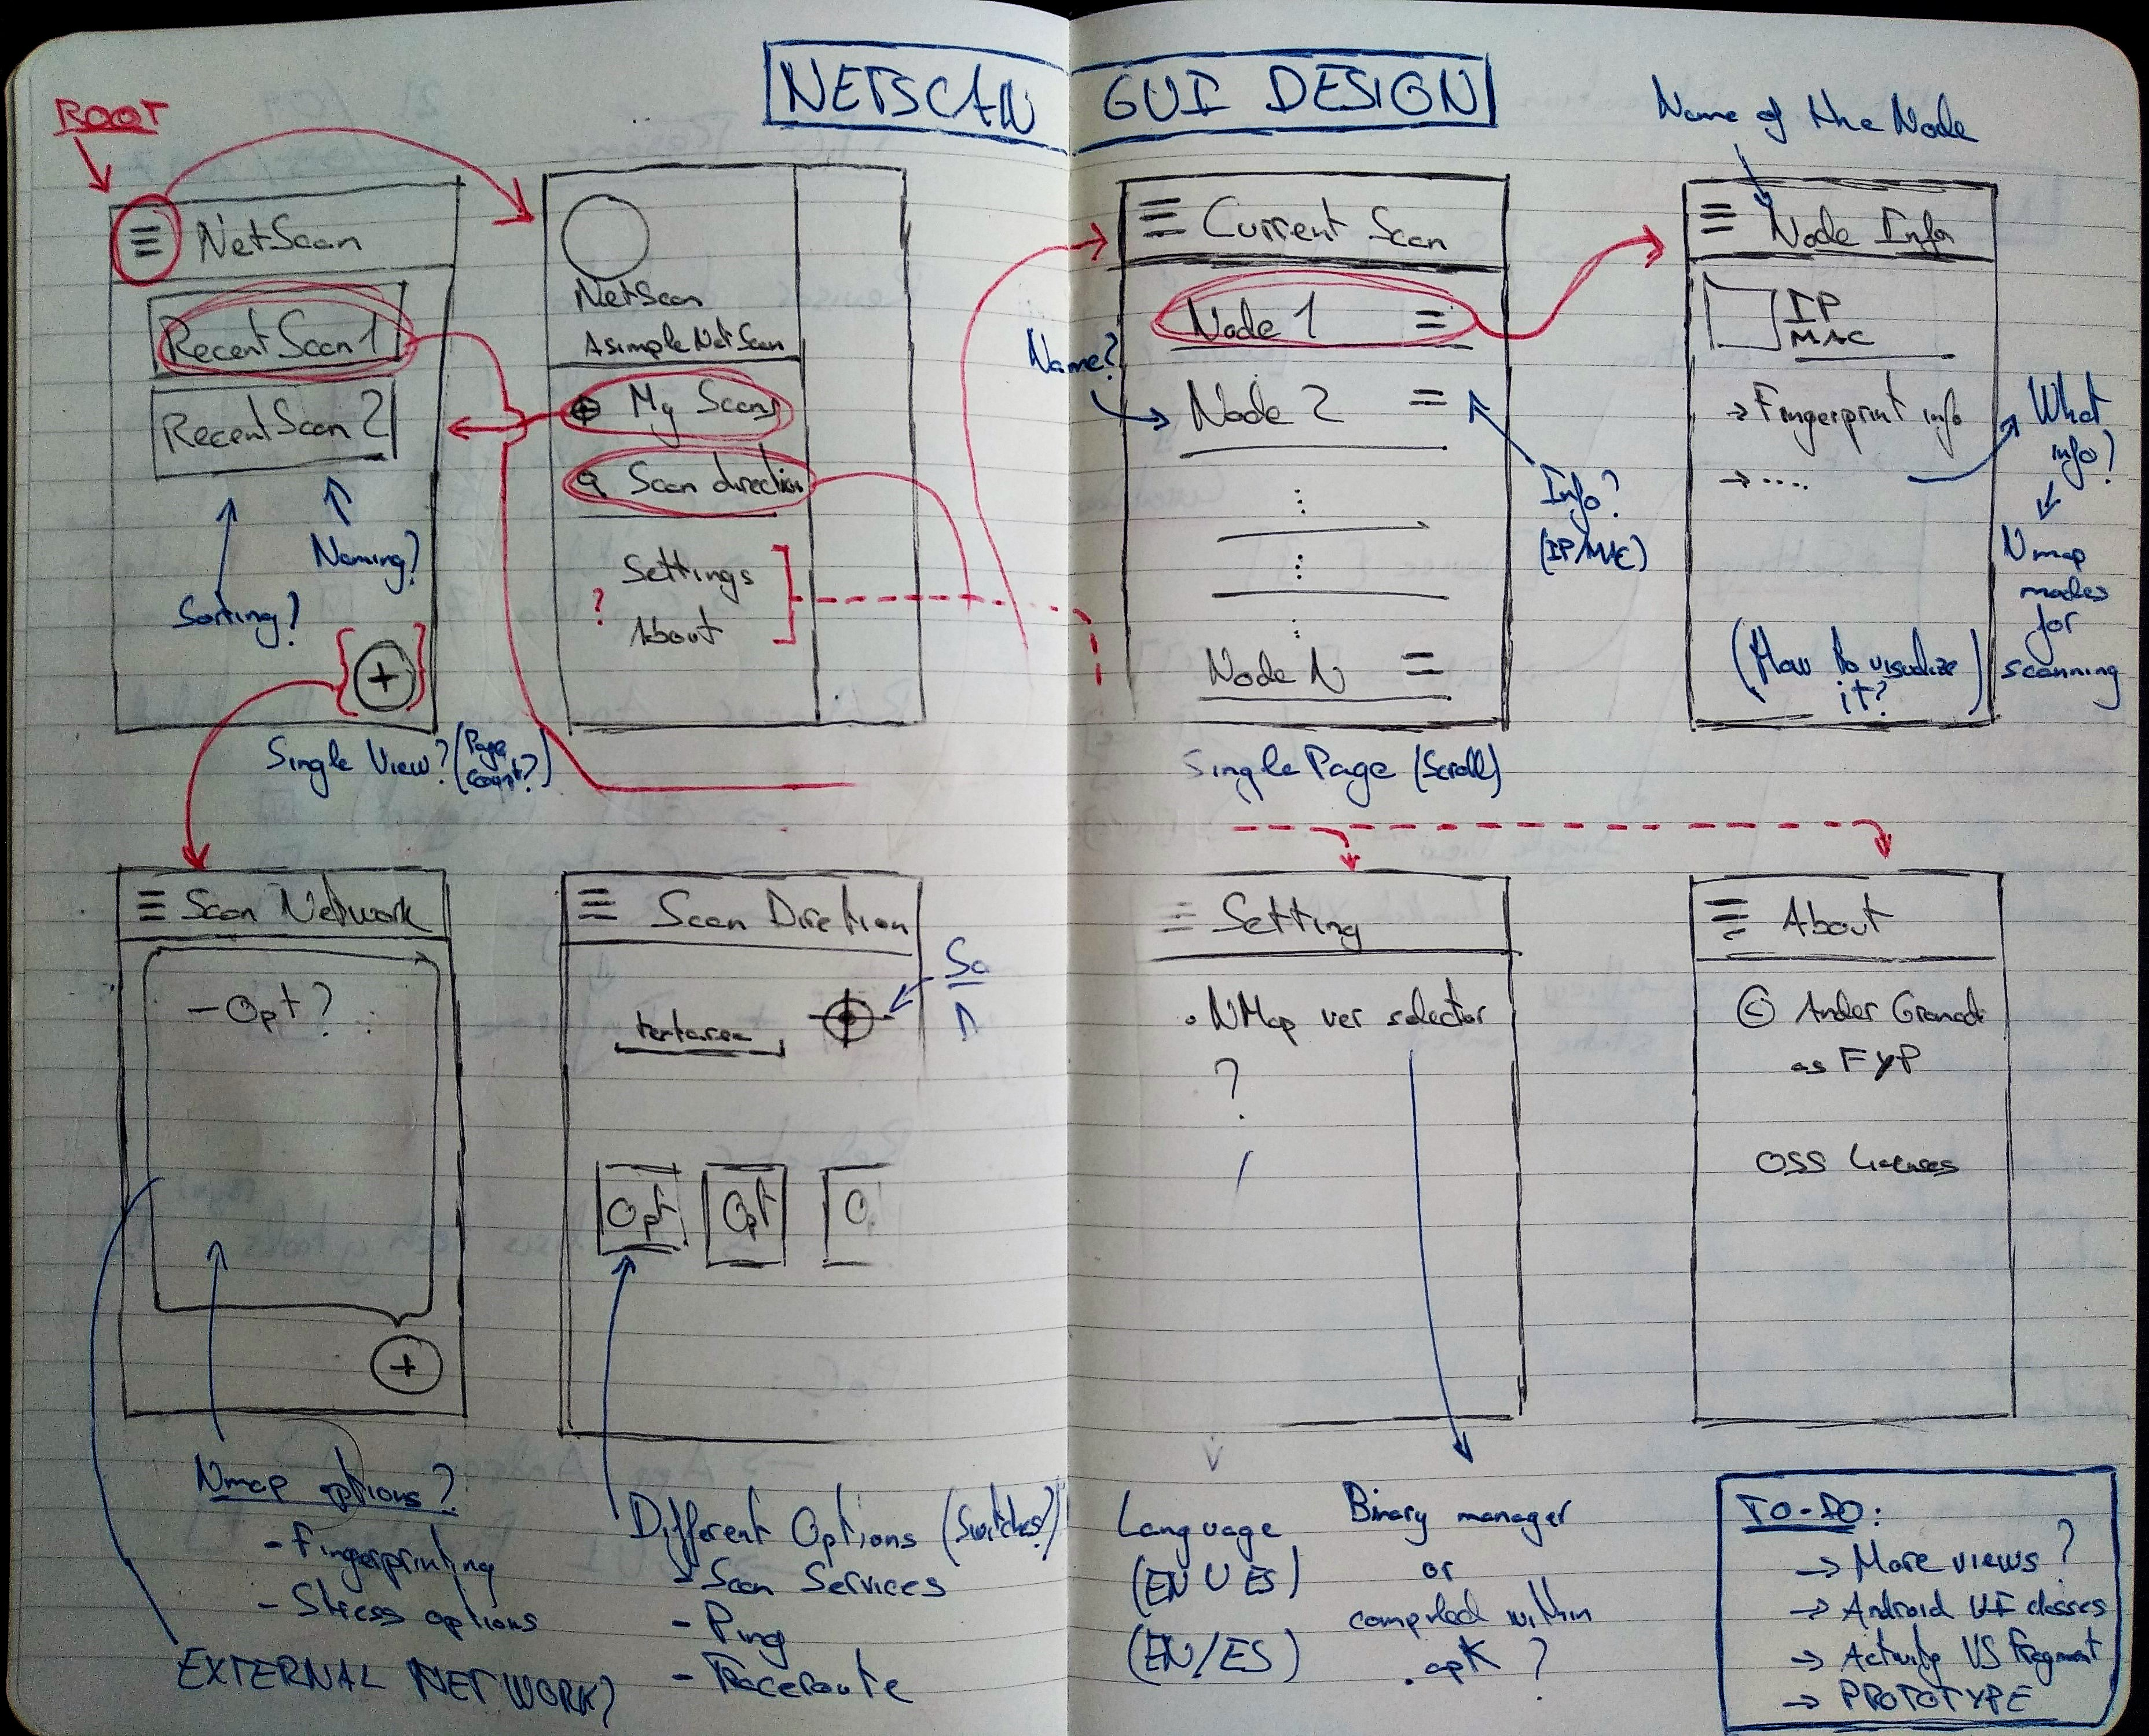
\includegraphics[width=\textwidth]{gui-mockup}
	\caption{Mockup inicial de la GUI de la aplicación}
	\label{fig:mockup}
\end{figure}

La aplicación esta dividida en varias vistas. Debido a que el objetivo principal de la aplicación es que sea lo mas simple posible, se ha diseñado buscando minimizar el numero de ventanas de la aplicación.

A la hora de crear las vistas en Android se usan dos conceptos. \textit{Activity} y \textit{Fragment}. En Android, una Activity representa una parte de la UI de una aplicación, y tiene su propio ciclo de vida y su propia jerarquía de elementos. Una aplicación Android dispone de tantas Activity como el usuario quiera implementar, entendiendo que cada Activity servirá para mostrar cierta información e interactúa con el usuario de una manera concreta. A continuación se muestra el ciclo de vida de una Activity, con los métodos que se ejecutan en ciertos puntos

\begin{figure}[H]
	\centering
	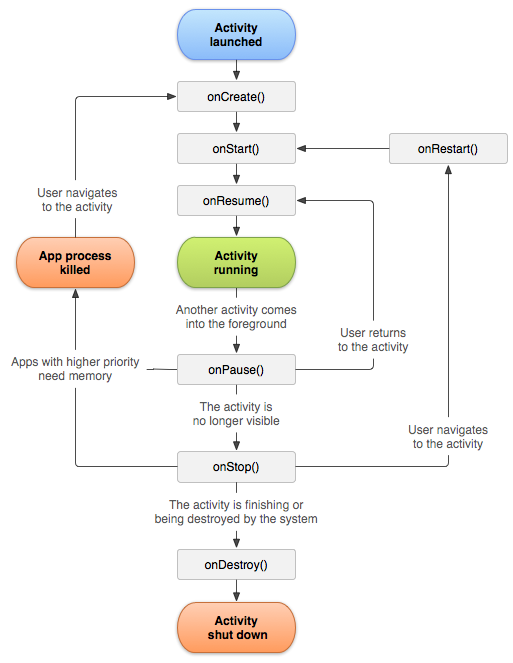
\includegraphics[width=0.75\textwidth]{activity-lc}
	\caption{Ciclo de vida de una Activity de Android}
	\label{fig:activity-lc}
\end{figure}

El Fragment, aunque también representa una parte de la UI de la aplicación, depende de una Activity, ya que debe acoplarse a una. A diferencia del Activity, se pueden mostrar varios Fragments a la vez. Hay que tener en cuenta que un Fragment, aun teniendo su propio ciclo de vida (más simplificado que el del Activity) depende del ciclo de vida del Activity al que este acoplado. 

\begin{figure}[H]
	\centering
	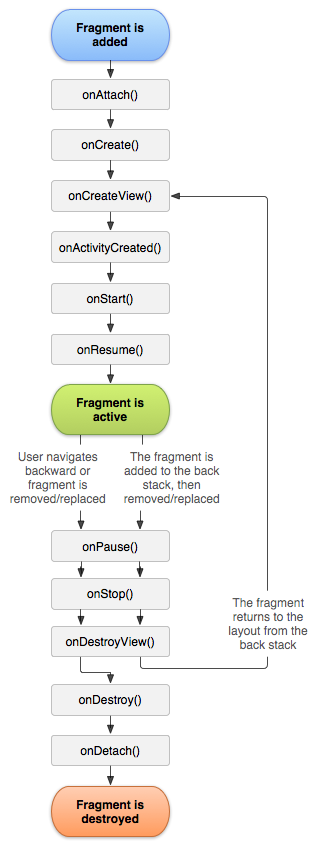
\includegraphics[height=0.75\textheight]{fragment-lc}
	\caption{Ciclo de vida de un Fragment de Android}
	\label{fig:fragment-lc}
\end{figure}


En Android, a la hora de diseñar aplicaciones, se usan Fragments para partes reutilizables y comunes de una UI y se usan las Activities para controlar el ciclo de vida de la aplicación. En una aplicación de Android abierta siempre se encuentra activa una Activity, que muestra algún tipo de interfaz.

La aplicación dispone de una serie Activities y Fragments implementados, cuya lista se muestra en la \autoref{fig:views-list}.

\begin{figure}[H]
	\centering
	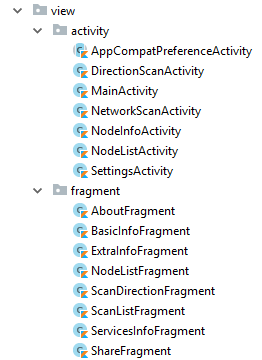
\includegraphics{views-list}
	\caption{Lista de clases con las Activities y Fragments implementados en la aplicación}
	\label{fig:views-list}
\end{figure}


{\color{red} Falta rellenar este capítulo, que básicamente consiste en explicar las diferentes partes de la aplicación, con capturas y referencias a elementos de diseño y Material Design}